\section{OJ 10077 -- The Stern-Brocot Number System}

\begin{frame}[fragile]{Problema}

The Stern-Brocot tree is a beautiful way for constructing the set of all nonnegative fractions 
$\frac{m}{n}$ where $m$ and $n$ are relatively prime. The idea is to start with two fractions 
$(\frac{0}{1}, \frac{1}{0})$ and then repeat the following operations as many times as desired:

\begin{center}
Insert $\frac{m+m'}{n+n'}$ between two adjacent fractions $\frac{m}{n}$ and $\frac{m'}{n'}$. 
\end{center}

For example, the first step gives us one new entry between $\frac{0}{1}$ and $\frac{1}{0}$,
\[
    \frac{0}{1}, \frac{1}{1}, \frac{1}{0}
\]
and the next gives two more:
\[
    \frac{0}{1}, \frac{1}{2}, \frac{1}{1}, \frac{2}{1},\frac{1}{0}
\]

\end{frame}

\begin{frame}[fragile]{Problema}
The next gives four more,
\[
    \frac{0}{1}, \frac{1}{3}, \frac{1}{2}, \frac{2}{3}, \frac{1}{1}, \frac{3}{2}, \frac{2}{1},
    \frac{3}{1},\frac{1}{0}
\]
and then we will get 8, 16, and so on. The entire array can be regarded as an infinite binary tree
structure whose top levels look like this:
\begin{figure}
    \centering
    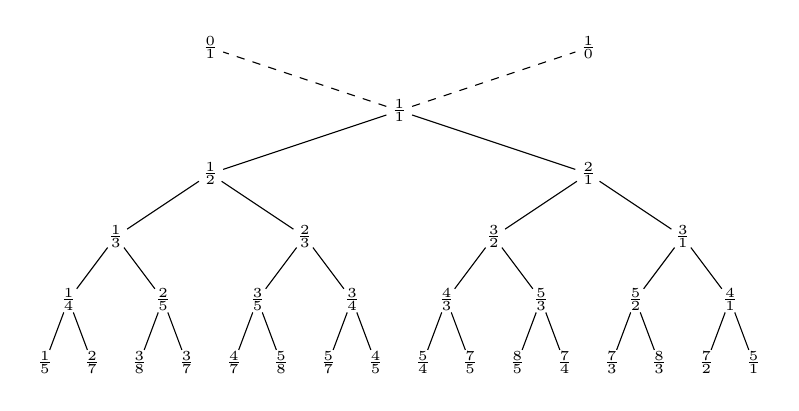
\begin{tikzpicture}
        \node[circle,fill,white] (A) at (0, 0) {};
        \node[circle,fill,white] (B) at (0.3, 0.8) {};
        \node[circle,fill,white] (C) at (0.6, 0) {};
        \node[circle,fill,white] (D) at (1.2, 0) {};
        \node[circle,fill,white] (E) at (1.5, 0.8) {};
        \node[circle,fill,white] (F) at (1.8, 0) {};
        \node[circle,fill,white] (G) at (2.4, 0) {};
        \node[circle,fill,white] (H) at (2.7, 0.8) {};
        \node[circle,fill,white] (I) at (3.0, 0) {};
        \node[circle,fill,white] (J) at (3.6, 0) {};
        \node[circle,fill,white] (K) at (3.9, 0.8) {};
        \node[circle,fill,white] (L) at (4.2, 0) {};
        \node[circle,fill,white] (M) at (4.8, 0) {};
        \node[circle,fill,white] (N) at (5.1, 0.8) {};
        \node[circle,fill,white] (O) at (5.4, 0) {};
        \node[circle,fill,white] (P) at (6.0, 0) {};
        \node[circle,fill,white] (Q) at (6.3, 0.8) {};
        \node[circle,fill,white] (R) at (6.6, 0) {};
        \node[circle,fill,white] (S) at (7.2, 0) {};
        \node[circle,fill,white] (T) at (7.5, 0.8) {};
        \node[circle,fill,white] (U) at (7.8, 0) {};
        \node[circle,fill,white] (V) at (8.4, 0) {};
        \node[circle,fill,white] (X) at (8.7, 0.8) {};
        \node[circle,fill,white] (Y) at (9.0, 0) {};

        \node[circle,fill,white] (A1) at (0.9, 1.6) { };
        \node[circle,fill,white] (B1) at (3.3, 1.6) { };
        \node[circle,fill,white] (C1) at (5.7, 1.6) { };
        \node[circle,fill,white] (D1) at (8.1, 1.6) { };

        \node[circle,fill,white] (A2) at (2.1, 2.4) { };
        \node[circle,fill,white] (B2) at (6.9, 2.4) { };

        \node[circle,fill,white] (A3) at (4.5, 3.2) { };

        \node[circle,fill,white] (A4) at (2.1, 4.0) { };
        \node[circle,fill,white] (B4) at (6.9, 4.0) { };

        \draw (A) -- (B);
        \draw (C) -- (B);
        \draw (D) -- (E);
        \draw (E) -- (F);
        \draw (G) -- (H);
        \draw (H) -- (I);
        \draw (J) -- (K);
        \draw (K) -- (L);
        \draw (M) -- (N);
        \draw (O) -- (N);
        \draw (P) -- (Q);
        \draw (R) -- (Q);
        \draw (S) -- (T);
        \draw (U) -- (T);
        \draw (V) -- (X);
        \draw (Y) -- (X);

        \draw (A1) -- (B);
        \draw (A1) -- (E);
        \draw (B1) -- (H);
        \draw (B1) -- (K);
        \draw (C1) -- (N);
        \draw (C1) -- (Q);
        \draw (D1) -- (T);
        \draw (D1) -- (X);

        \draw (A2) -- (A1);
        \draw (A2) -- (B1);
        \draw (B2) -- (C1);
        \draw (B2) -- (D1);

        \draw (A3) -- (A2);
        \draw (A3) -- (B2);

        \draw[dashed] (A3) -- (A4);
        \draw[dashed] (A3) -- (B4);
        \node at (0, 0) { \tiny $\frac{1}{5}$ };
        \node at (0.6, 0) { \tiny $\frac{2}{7}$ };
        \node at (1.2, 0) { \tiny $\frac{3}{8}$ };
        \node at (1.8, 0) { \tiny $\frac{3}{7}$ };
        \node at (2.4, 0) { \tiny $\frac{4}{7}$ };
        \node at (3.0, 0) { \tiny $\frac{5}{8}$ };
        \node at (3.6, 0) { \tiny $\frac{5}{7}$ };
        \node at (4.2, 0) { \tiny $\frac{4}{5}$ };
        \node at (4.8, 0) { \tiny $\frac{5}{4}$ };
        \node at (5.4, 0) { \tiny $\frac{7}{5}$ };
        \node at (6.0, 0) { \tiny $\frac{8}{5}$ };
        \node at (6.6, 0) { \tiny $\frac{7}{4}$ };
        \node at (7.2, 0) { \tiny $\frac{7}{3}$ };
        \node at (7.8, 0) { \tiny $\frac{8}{3}$ };
        \node at (8.4, 0) { \tiny $\frac{7}{2}$ };
        \node at (9.0, 0) { \tiny $\frac{5}{1}$ };

        \node at (0.3, 0.8) { \tiny $\frac{1}{4}$ };
        \node at (1.5, 0.8) { \tiny $\frac{2}{5}$ };
        \node at (2.7, 0.8) { \tiny $\frac{3}{5}$ };
        \node at (3.9, 0.8) { \tiny $\frac{3}{4}$ };
        \node at (5.1, 0.8) { \tiny $\frac{4}{3}$ };
        \node at (6.3, 0.8) { \tiny $\frac{5}{3}$ };
        \node at (7.5, 0.8) { \tiny $\frac{5}{2}$ };
        \node at (8.7, 0.8) { \tiny $\frac{4}{1}$ };

        \node at (0.9, 1.6) { \tiny $\frac{1}{3}$ };
        \node at (3.3, 1.6) { \tiny $\frac{2}{3}$ };
        \node at (5.7, 1.6) { \tiny $\frac{3}{2}$ };
        \node at (8.1, 1.6) { \tiny $\frac{3}{1}$ };

        \node at (2.1, 2.4) { \tiny $\frac{1}{2}$ };
        \node at (6.9, 2.4) { \tiny $\frac{2}{1}$ };

        \node at (4.5, 3.2) { \tiny $\frac{1}{1}$ };

        \node at (2.1, 4.0) { \tiny $\frac{0}{1}$ };
        \node at (6.9, 4.0) { \tiny $\frac{1}{0}$ };

    \end{tikzpicture}
\end{figure}
\end{frame}

\begin{frame}[fragile]{Problema}
The construction preserves order, and we couldn’t possibly get the same fraction in two 
different places.

We can, in fact, regard the Stern-Brocot tree as a number system for representing rational numbers,
because each positive, reduced fraction occurs exactly once. Let’s use the letters ‘\texttt{L}’ 
and ‘\texttt{R}’ to stand for going down to the left or right branch as we proceed from the root 
of the tree to a particular fraction; then a string of \texttt{L}’s and \texttt{R}’s uniquely 
identifies a place in the tree. For example, \texttt{LRRL} means that we go left from $\frac{1}{1}$
down to $\frac{1}{2}$, then right to $\frac{2}{3}$, then right to $\frac{3}{4}$, then left to 
$\frac{5}{7}$. We can consider \texttt{LRRL} to be a representation of $\frac{5}{7}$. Every 
positive fraction gets represented in this way as a unique string of \texttt{L}’s and 
\texttt{R}’s.

\end{frame}

\begin{frame}[fragile]{Problema}
Well, actually there’s a slight problem: The fraction $\frac{1}{1}$ corresponds to the empty 
string, and we need a notation for that. Let’s agree to call it \texttt{I}, because that looks 
something like 1 and it stands for \lq\lq identity\rq\rq.

In this problem, given a positive rational fraction, you are expected to represent it in 
\textit{Stern-Brocot number system}.
\end{frame}

\begin{frame}[fragile]{Entrada e saída}

\textbf{Input}

The input file contains multiple test cases. Each test case consists of a line contains two 
positive integers $m$ and $n$ where $m$ and $n$ are relatively prime. The input terminates with a 
test case containing two 1’s for $m$ and $n$, and this case must not be processed.

\vspace{0.1in}

\textbf{Output}

For each test case in the input file output a line containing the representation of the given 
fraction in the \textit{Stern-Brocot number system}.

\end{frame}

\begin{frame}[fragile]{Exemplo de entradas e saídas}

\begin{minipage}[t]{0.5\textwidth}
\textbf{Exemplo de Entrada}
\begin{verbatim}
5 7
878 323
1 1
\end{verbatim}
\end{minipage}
\begin{minipage}[t]{0.45\textwidth}
\textbf{Exemplo de Saída}
\begin{verbatim}
LRRL
RRLRRLRLLLLRLRRR
\end{verbatim}
\end{minipage}
\end{frame}

\begin{frame}[fragile]{Solução}

    \begin{itemize}
        \item A árvore apresentada no exemplo e as sequências iniciais permitem a observação
            que a árvore com raiz $\frac{1}{1}$ é uma árvore binária de busca

        \item Este fato permite o uso da busca binária para determinar, a cada elemento, se é 
            preciso seguir à esquerda ou à direita

        \item A busca se encerra quando o número a ser representado é atingido

        \item Deste modo, a solução tem complexidade $O(H)$, onde $H$ é o número
            de elementos que compõem a representam da fração $n/m$ no sistema apresentado
   \end{itemize}

\end{frame}

\begin{frame}[fragile]{Solução $O(H)$}
    \inputsnippet{cpp}{1}{21}{codes/10077.cpp}
\end{frame}

\begin{frame}[fragile]{Solução $O(H)$}
    \inputsnippet{cpp}{23}{43}{codes/10077.cpp}
\end{frame}

\begin{frame}[fragile]{Solução $O(H)$}
    \inputsnippet{cpp}{44}{64}{codes/10077.cpp}
\end{frame}
